%!TEX program = lualatex
%!TEX encoding = UTF-8 Unicode  
%!TEX root = chapter04.tex  
\documentclass[main.tex]{subfiles} 
\begin{document} 
%----------------------------------------------------------------------------------------
%	CHAPTER 4
%----------------------------------------------------------------------------------------
\cleardoublepage 
\loadgeometry{marginlayout}  
\pagestyle{scrheadings} % Print headers again  
\KOMAoptions{
headwidth=textwithmarginpar,
headsepline=true,
headsepline= 0.5pt,
footwidth=textwithmarginpar,
}   
\onehalfspacing 
\setcounter{chapter}{3}
\chapter{Transformations rigides de figures}
 
\section{La symétrie axiale} 
Transformer une figure par \textbf{symétrie axiale}, c'est la retourner en pliant le long d'un axe. 
\begin{figure}[h]
	\begin{tikzpicture}[scale=0.5]
		\tkzDefPoints{1.5/-1.5/C,-4.5/2/D}
		\tkzDefPoint(-4,-2){O}
		\tkzDefPoint(-2,-2){A}
		\foreach \i in {0,1,...,4}{%
			\pgfmathparse{0+\i * 72}
			\tkzDefPointBy[rotation=%
			center O angle \pgfmathresult](A)
			\tkzGetPoint{A\i}
			\tkzDefPointBy[reflection = over C--D](A\i)
			\tkzGetPoint{A\i'}}
		\tkzDrawPolygon(A0, A2, A4, A1, A3)
		\tkzDrawPolygon(A0', A2', A4', A1', A3')
		\tkzDrawLine[add= .5 and .5](C,D)
	\end{tikzpicture}
\end{figure} 
Les deux figures symétriques doivent se superposer parfaitement après un pliage le long de l'axe de symétrie.
\marginpar{ 
	\captionsetup{type=figure}\centering
	\begin{tikzpicture}[scale=0.75]
		\tkzInit[ymin=-4,ymax=4.5,xmin=-6,xmax=2]
		\tkzClip
		\tkzDefPoints{1.5/-1.5/C,-4.5/2/D}
		\tkzDefPoint(-4,-2){A}
		%\tkzDefPoint(-2,-2){B}
		\tkzDefPointBy[reflection = over C--D](A) \tkzGetPoint{A'}
		\tkzInterLL(A,A')(C,D) \tkzGetPoint{I}
		\tkzDrawPoints(A,A',I)
		\tkzLabelPoint[above](I){$I$}
		\tkzLabelPoint(A){$M$}
		\tkzLabelPoint(A'){$M'$}
		\tkzDrawSegment(A,A')
		\tkzDrawSegments[dashed, color=red](C,A C,A')
		\tkzDrawSegments[dashed, color=blue](D,A D,A')
		\tkzMarkSegments[mark=s|](C,A C,A')
		\tkzMarkSegments[mark=s](D,A D,A')
		\tkzMarkSegments[mark=s||](A,I I,A')
		\tkzMarkRightAngle[fill=lightgray](A,I,C)
		\tkzCompass[color=red,length=1.5](C,A)
		\tkzCompass[color=red,length=1.5](C,A')
		\tkzCompass[color=blue,length=1.5](D,A)
		\tkzCompass[color=blue,length=1.5](D,A')
		\tkzDrawLine[add= .2 and .2](C,D)
		\tkzLabelLine[pos=1.2, right](C,D){$\Delta$}
	\end{tikzpicture}
	\caption{$M'$ est le symétrique de $M$ par rapport à $\Delta$}	
}
\begin{definition}
	Les points $M'$ et $M$ sont symétriques par rapport à l'axe $\Delta$ lorsque $\Delta$ est la \textbf{médiatrice} du segment $[MM']$.
	
	L'image d'un point de $\Delta$ par la symétrie d'axe $\Delta$ est lui-même.  
\end{definition}
%%%%%%%%%%%%%%%%%%%%%%%%%%%%%%%%%%%%%%%%%%%%%%%%%%%%%%%%%%%
%
%%%%%%%%%%%%%%%%%%%%%%%%%%%%%%%%%%%%%%%%%%%%%%%%%%%%%%%%%%%
\newpage 
\section{La translation} 
\marginpar{
	\captionsetup{type=figure}\centering
	\begin{tikzpicture}[>=latex, scale=0.8]
		\tkzDefPoint(0,0){A} \tkzDefPoint(3,1){A'}
		\tkzDefPoint(3,0){B} \tkzDefPoint(1,2){C}
		\tkzDefPointsBy[translation= from A to A'](B,C){}
		\tkzDrawPolygon[color=blue](A,B,C)
		\tkzDrawPolygon[color=red](A',B',C')
		\tkzDrawPoints[color=blue](A,B,C)
		\tkzDrawPoints[color=red](A',B',C')
		\tkzLabelPoints(A,B,A',B')
		\tkzLabelPoints[above](C,C')
		\tkzDrawSegments[color = gray,->,
		style=dashed](A,A' B,B' C,C')
	\end{tikzpicture}
	\caption[Translation]{La translation de vecteur $\vv{AA'}$, transforme le triangle $ABC$ en $A'B'C'$.}
} 
Transformer une figure par translation, c’est la glisser sans la tourner. 
\begin{definition}
	Une translation de vecteur $\vv{PQ}$ lorsqu'elle transforme le point $P$ en $Q$.
	
	La translation est caractérisée par :
	\begin{description} 
		\item[une \textbf{direction}] parallèle à la droite $(PQ)$
		%discuter de la différence entre direction en mathématique et direction dans l'usage courant. en utilisant l'image des lignes TGV.
		\item[un \textbf{sens}] de $P$ vers $Q$.
		\item[une \textbf{longueur}] la longueur $PQ$.
	\end{description} 
\end{definition}
Les phrases suivantes sont synonymes :
\begin{itemize}[label=\textbullet, left=-0.2em]
	\item  $A'$ est l'image de $A$ par la translation de vecteur $\vv{PQ}$ 
	\item   $A'$ est l'image de $A$ par la translation qui transforme $P$ en $Q$ 
	\item   $Q$ est l'image de $P$ par la translation qui transforme $A$ en $A'$ 
	\item   $AA'QP$ est un parallélogramme
\end{itemize}  
%Les translations de vecteur $\vv{AA'}$ et $\vv{PQ}$ sont identiques. On peut écrire $\vv{AA'}=\vv{PQ}$.
\begin{example}Quelques translations 
	\begin{figure}[hb]
		\begin{tikzpicture}[scale=0.45]
			\tkzInit[xmin=-8,xmax=15,ymin=-9,ymax=5  ]
			\begin{scope}[dotted]
				\tkzGrid[color=gray](-8,-9)(15,5)
			\end{scope}
			\tkzSetUpPoint[size=2, fill=black]
			\tkzfctset{tan style/.style={->,>=latex, color=red, line width=1.2pt}} 
			
			
			\filldraw[draw=black, line width=2pt] 
			(3,-1) circle (2pt) node[align=center, below] {}     -- 
			(3,0) circle (2pt) node[align=center, below] {}     -- 
			(5,0) circle (2pt) node[align=center, below] {}     -- 
			(5,-3) circle (2pt) node[align=right,  below] {}  -- 
			(7,-3) circle (2pt) node[align=right,  below] {}  -- 
			(7,-4) circle (2pt) node[align=right,  below] {}  -- 
			(6,-5) circle (2pt) node[align=right,  below] {} -- 
			(2,-5) circle (2pt) node[align=center, below] {} -- 
			(1,-4) circle (2pt) node[align=center, below] {} -- 
			(2,-3) circle (2pt) node[align=center, below] {}  -- 
			(5,-3) circle (2pt) node[align=center, below] {}  -- 
			(5,-1) circle (2pt) node[align=center, below] {} -- 
			(3,-1) circle (2pt) node[align=center, below] {};
			
			
			
			\tkzDefPoint(-6,-3){P}
			\tkzDefPoint(-1,-6){Q}
			\tkzDrawPoints(P,Q) 
			\tkzLabelPoint[above](P){$A$}
			\tkzLabelPoint(Q){$B$}
			
			%		\tkzDefPoint(-7,3){S}
			%		\tkzDefPoint(-1,9){T}
			%		\tkzDrawPoints(S,T) 
			%		\tkzLabelPoint[above](S){$S$}
			%		\tkzLabelPoint(T){$T$}	
			%		\tkzDrawSegments[->,>=latex, line width= 1pt](S,T) 
		\end{tikzpicture}
		\caption[Exemple translation 1]{Tracer en bleu l'image de la figure par la translation qui transforme $A$ et $B$. 
			Tracer en rouge l'image de la figure par la translation de vecteur $\vv{BA}$.
		}
	\end{figure}
	%\begin{exampleT} Tracer l'image du triangle par la translation de vecteur $\vv{BA}$.
	\begin{figure}[hb]
		\begin{tikzpicture}[scale=0.70]
			\tkzSetUpPoint[size=3, fill=black]
			\tkzfctset{tan style/.style={->,>=latex, color=red, line width=1.2pt}} 
			\tkzDefPoint(2.5,5.5){A} 
			\tkzDefPoint(5.25,4.2){B}
			\tkzDefPoint(0,3.5){C}
			\tkzDefPoint(-1.7,0.25){D}
			\tkzDefPoint(2.8,0.6){E}
			\tkzDrawPolygon[ line width=1.0pt, fill=gray!05](C,D,E) 
			\tkzDrawPoints(A,B) 
			\tkzLabelPoint[below left](A){\scriptsize$A$}
			\tkzLabelPoint[below left](B){\scriptsize$B$} 
			\tkzDefPointsBy[translation= from A to B](E){E'}
			\tkzDefPoint(0,6){U} 
			\tkzDefPoint(0,-2){V} 
		\end{tikzpicture} 
		\caption[Exemple translation 2]{Tracer l'image du triangle par la translation qui transforme $B$ en $A$.}
	\end{figure}
\end{example} 

%%%%%%%%%%%%%%%%%%%%%%%%%%%%%%%%%%%%%%%%%%%%%%%%%%%%%%%%%%%
%
%%%%%%%%%%%%%%%%%%%%%%%%%%%%%%%%%%%%%%%%%%%%%%%%%%%%%%%%%%%
\clearpage
\section{La rotation} 
Transformer une figure par rotation c'est la faire tourner autour d'un point.
\marginpar{
	\captionsetup{type=figure}\centering
	\begin{tikzpicture}
		\tkzDefPoint(0,0){O}
		\tkzDefPoint(3,1){M}
		\tkzDefPointBy[rotation= center O angle 55](M) \tkzGetPoint{M'}
		\tkzDrawPoints(O,M,M')
		\tkzDrawSegments(O,M O,M')
		\tkzMarkAngle[size=0.5, fill=blue!20, opacity=0.6, mark=none](M,O,M')
		\tkzMarkSegments[mark=s||](O,M O,M')
		\tkzLabelAngle[pos=0.7](M,O,M'){$\alpha$}
		\tkzLabelPoint[left,color=black](O){$O$}
		\tkzLabelPoint[right,color=black](M){$M$}
		\tkzLabelPoint[left,color=black](M'){$M'$}
		\draw[red, ->,>=latex] (2.7,1.8) arc (40:60:3);
		\tkzText[fill=White,draw=black, text width=2cm](3,3.75){\scriptsize Sens direct (anti-horaire)}
	\end{tikzpicture}
	\caption{$M'$ est l'image de $M$ par la rotation de centre $O$, de sens direct (anti-horaire) et d'angle $\alpha$.}
}
\begin{definition}
	Pour caractériser une rotation il faut préciser :
	\begin{itemize}[label=\textbullet, left=0em]
		\item \textbf{son centre de rotation $0$}
		\item \textbf{son sens de rotation} : anti-horaire et horaire.
		\item \textbf{son angle de rotation $\alpha$}
	\end{itemize}
\end{definition}
\begin{example} Rotations d'angle \ang{90} et \ang{70}.
	\begin{figure}[hb] 
		\begin{tikzpicture}[scale=0.85]
			\tikzset{
				dot/.style 2 args={fill, cross out , draw   ,  inner sep=0pt, label={[label  distance=0pt]#1:\tiny #2}}
			}
			\def\numberlist{{3,0,1,0,2,3,0,2,1,404,2,1,0,6,7,1,1,3,4,5,1,3,2,1,0}}   
			\def\maxX{10}
			\foreach \x [count=\n] in {0,...,\maxX}{
				\foreach \y in {0,...,10}{
					\pgfmathtruncatemacro\tmp{\n+(\maxX+1)*\y}
					\pgfmathtruncatemacro\num{\tmp-1}
					\draw[line width=.5pt, dotted] (\x,0) -- (\x,10);
					\draw[line width=.5pt, dotted] (0,\y) -- (\maxX,\y);
					%			\node[dot={45}{\num}] at (\x,\y) {};
				}
			}
			\tkzDefPoint(2,8){B}
			\tkzDefPoint(4,3){A}
			\tkzDrawPoints[circle, size=4](A,B)
			\tkzLabelPoints(A,B)
			
			\tkzDefPoints{3/3/C,4/3/D,4/7/E,3/7/F,3/6/G,4/6/H}
			\tkzDrawPolygon[line width=2pt](C,D,E,F,G,H)
		\end{tikzpicture}
		\caption[Exemple de rotation 1]{Tracer en bleu l'image de la figure par la rotation de centre $A$ et d'angle $\ang{90}$ dans le sens horaire. Tracer en rouge l'image de la figure par la rotation de centre $B$ et d'angle $\ang{90}$ dans le sens anti-horaire.}
	\end{figure} 
	\begin{figure}[hb] 
		\begin{tikzpicture}[scale=0.80]
			\tkzDefPoint(-5,0){OO}
			\tkzDefPoint(0,0){O}
			\tkzLabelPoint(O){$O$}
			\tkzDefPoint(3,1){A}
			\tkzDefShiftPoint[A](-15:2.5){B}
			\tkzDefShiftPoint[A](75:4.1){C}
			\tkzDrawPoints(A,B,C,O)
			\tkzDrawPolygon(A,B,C)
			\tkzFillPolygon[color=yellow, opacity=.2](A,B,C)
			\tkzDefPointBy[rotation= center O angle 70](A) \tkzGetPoint{A'}
			\tkzDefPointBy[rotation= center O angle 70](B) \tkzGetPoint{B'}
			\tkzDefPointBy[rotation= center O angle 70](C) \tkzGetPoint{C'}
			\tkzMarkRightAngle[size=0.2](C,A,B)
			%\tkzDrawPoints[color=white](A',B',C') 
			\tkzDefShiftPoint[C'](0,1){C''}
			\tkzDrawSegment[color=red,line width=1pt](O,B)
			\tkzDrawLine[color=red,line width=1pt, add = 0 and .2](O,B') %,end=$[AB)$
			%			\tkzProtractor[scale=0.8,with=half](O,B)
			\tkzCompass[color=red,length=1.5](O,B)
			\tkzCompass[color=red,length=1.5](O,B')
			\tkzLabelPoint[below right](B){$B$}
			\tkzLabelPoint[above left](B'){$B'$}
			\tkzMarkAngle[size=0.5, fill=red!20, opacity=0.6](B,O,B')
			\tkzLabelAngle[pos=0.9, mark=none](B,O,B'){\ang{70}}
			
		\end{tikzpicture}
		\caption[Exemple de rotation 2]{Tracer l'image du triangle rectangle $ABC$ par la rotation de centre $O$ et d'angle $\ang{70}$ dans le sens anti-horaire.}
	\end{figure}
\end{example}
 

%----------------------------------------------------------------------------------------
%	EXERCICES
%----------------------------------------------------------------------------------------

\newpage 
\loadgeometry{widelayout}  
\pagestyle{scrheadings} % Print headers again  
\KOMAoptions{
headwidth=textwithmarginpar,
headsepline=true,
headsepline= 0.5pt,
footwidth=textwithmarginpar,
} 
\onehalfspacing
\section{Exercices}


\begin{figure}[h]
	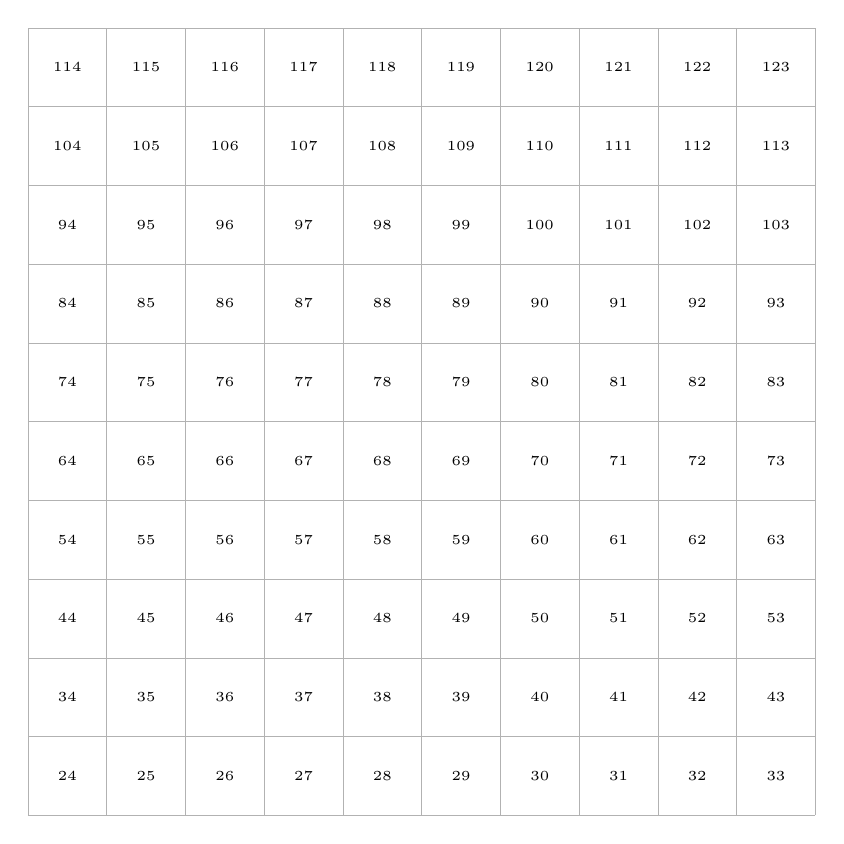
\begin{tikzpicture}
		\draw[very thin, black!30] (0,0) grid (10,10);
		
		\foreach \y in {9,...,0}
		\foreach \x in {1,...,10}
		\pgfmathsetmacro\z{int(23+\x+(10*\y))}
		\node  at (\x-0.5,\y+0.5) {\tiny\z};
		\tkzDefPoint(1,2){B}
		\tkzDefPoint(2,10){A}
		\tkzDefPoint(7,6){C}
		\tkzDefPoint(3,4){D}
		\tkzDefPoint(5,4){E}
		\tkzDrawPoints[circle, size=4](A,B,C,D,E)
		\tkzLabelPoints[right](A,B,C,D,E)
	\end{tikzpicture}
\end{figure}
\begin{exercise} \hfill 
	\begin{enumerate}[label=\arabic*),leftmargin=*]
		\item Quel est le numéro de la figure image de la figure 54 par la rotation de centre $A$ et d'angle \ang{90} dans le sens  direct ?
		\item Quel est le numéro de la figure image de la figure 29 par la rotation de centre $B$ et d'angle \ang{90} dans le sens anti-horaire ?
		\item Quel est le numéro  de la figure image de la figure 48 par la rotation de centre $C$ et d'angle \ang{90} dans le sens indirect ?
		\item Quel est le numéro de la figure image de la figure 110 par la rotation de centre $D$ et d'angle \ang{90} dans le sens horaire ?
		\item Quel est le numéro de la figure image de la figure 69 par la rotation de centre $E$ et d'angle \ang{90} dans le sens inverse des aiguilles d'une montre ?
	\end{enumerate}
\end{exercise}
\begin{exercise} \hfill 
	\begin{enumerate}[label=\arabic*),leftmargin=*]
		\item  Dans la translation qui transforme la figure 63 en la figure 120, quelle est l'image de la figure 58 ?
		\item  Dans la translation qui transforme la figure 43 en la figure 89, quelle est l'image de la figure 58 ?
		\item  Dans la translation qui transforme la figure 85 en la figure 98, quelle est l'image de la figure 58 ?
		\item Quelle est l'image de la figure 36 par la translation de vecteur $\vv{BE}$ ?
		\item Quelle est l'image de la figure 98 par la translation de vecteur $\vv{AC}$ ?
		\item Quelle est l'image de la figure 40 par la translation de vecteur $\vv{EC}$ ? 
	\end{enumerate}
\end{exercise}
\newpage 


\begin{exercise}[Brevet]   (  environ 10~\si{\minute})
	
	\parbox[t]{0.65\columnwidth}{\medskip
		\textbf{Dans cet exercice, aucune justification n'est attendue}
		
		On considère l'hexagone ABCDEF de centre $O$ représenté ci-contre.
		\begin{enumerate}[label=\arabic*),leftmargin=*]
			\item  Parmi les propositions suivantes, recopier celle qui correspond à l'image du quadrilatère CDEO par la symétrie de centre O.
			\renewcommand{\arraystretch}{1.5}
			\begin{tabularx}{\linewidth}{|*{3}{>{\centering \arraybackslash} X|}} \hline
				\textbf{Proposition 1}&\textbf{Proposition 2}&\textbf{Proposition 3}\\ \hline
				FABO & ABCO & FODE\\ \hline
			\end{tabularx}
		\end{enumerate}
	}
	\hfill 
	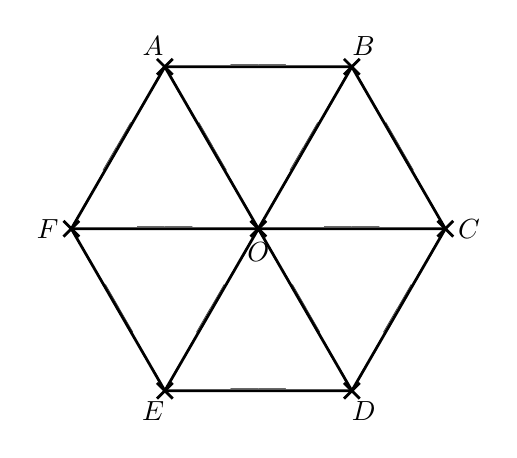
\begin{tikzpicture}[x=25mm,y=25mm,baseline={(A)},line width=1pt, scale=0.95]
		\newcommand{\point}[3]{\draw[shift={#1}] (-3pt,-3pt)--(3pt,3pt) (-3pt,3pt)--(3pt,-3pt) (0,0) node[shift={#2}]{#3};}
		
		\coordinate (A) at (120:1); \point{(A)}{(120:3mm)}{$A$};
		\coordinate (B) at ( 60:1); \point{(B)}{( 60:3mm)}{$B$};
		\coordinate (C) at (  0:1); \point{(C)}{(  0:3mm)}{$C$};
		\coordinate (D) at (300:1); \point{(D)}{(300:3mm)}{$D$};
		\coordinate (E) at (240:1); \point{(E)}{(240:3mm)}{$E$};
		\coordinate (F) at (180:1); \point{(F)}{(180:3mm)}{$F$};
		\coordinate (O) at (0 , 0); \point{(O)}{(270:3mm)}{$O$};
		
		\draw (A)--(B) node[pos=0.5,sloped]{||}
		--(C) node[pos=0.5,sloped]{||}
		--(D) node[pos=0.5,sloped]{||}
		--(E) node[pos=0.5,sloped]{||}
		--(F) node[pos=0.5,sloped]{||}
		--cycle node[pos=0.5,sloped]{||}
		(A)--(O) node[pos=0.5,sloped]{||}
		(B)--(O) node[pos=0.5,sloped]{||}
		(C)--(O) node[pos=0.5,sloped]{||}
		(D)--(O) node[pos=0.5,sloped]{||}
		(E)--(O) node[pos=0.5,sloped]{||}
		(F)--(O) node[pos=0.5,sloped]{||};
	\end{tikzpicture}
	
	\begin{enumerate}\setcounter{enumi}{1}
		%	\item  Parmi les propositions suivantes, recopier celle qui correspond à l'image du quadrilatère CDEO par la symétrie de centre O.
		%	
		%\renewcommand{\arraystretch}{1.5}
		%\begin{tabularx}{\linewidth}{|*{3}{>{\centering \arraybackslash} X|}} \hline
		%		\textbf{Proposition 1}&\textbf{Proposition 2}&\textbf{Proposition 3}\\ \hline
		%		FABO & ABCO & FODE\\ \hline
		%	\end{tabularx}
		%		
		\item Quelle est l'image du segment [AO] par la symétrie d'axe (CF) ?
		
		\item  On considère la rotation de centre O qui transforme le triangle OAB en le triangle OCD.
		
		Quelle est l'image du triangle BOC par cette rotation ?
	\end{enumerate}
	\parbox{11cm}{La figure ci-contre représente un pavage dont le motif de base a la même forme que l'hexagone ci-dessus.
		On a numéroté certains de ces hexagones.
		\begin{enumerate}\setcounter{enumi}{3}
			\item Quelle est l'image de l'hexagone 14 par la translation qui transforme l'hexagone 2 en l'hexagone 12 ?
	\end{enumerate}}\hfill 
	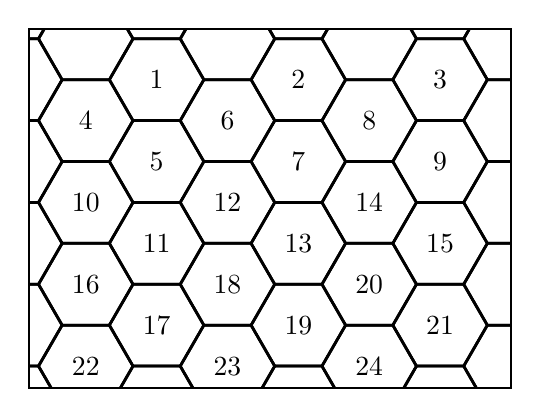
\begin{tikzpicture}[x=0.6cm,y=0.6cm,line width=1pt,baseline={(current bounding box.center)}]
		%\draw[teal,xstep=1,ystep=1] (0,0) grid (10,10);
		\clip[draw] (0.3,0.4) rectangle (10.5,8);
		\foreach \x  in {0,...,3}{
			\foreach \y in {0,...,5}
			\draw[shift={({3*\x},{1.732*\y})}] (0:1)--(60:1)--(120:1)--(180:1)--(240:1)--(300:1)--cycle (0,0);}
		\foreach \x  in {0,...,3}{
			\foreach \y in {0,...,5}
			\draw[shift={({1.5+3*\x},{0.866+1.732*\y})}] (0:1)--(60:1)--(120:1)--(180:1)--(240:1)--(300:1)--cycle;}
		\node at(3,6.928) {1}; \node at(6,6.928) {2}; \node at(9,6.928) {3};
		\node at(3,5.196) {5}; \node at(6,5.196) {7}; \node at(9,5.196) {9};
		\node at(3,3.464) {11}; \node at(6,3.464) {13}; \node at(9,3.464) {15};
		\node at(3,1.732) {17}; \node at(6,1.732) {19}; \node at(9,1.732) {21};
		\node at(1.5,6.062){4}; \node at(4.5,6.062){6}; \node at(7.5,6.062){8};
		\node at(1.5,4.33){10}; \node at(4.5,4.33){12}; \node at(7.5,4.33){14};
		\node at(1.5,2.598){16}; \node at(4.5,2.598){18}; \node at(7.5,2.598){20};
		\node at(1.5,0.866){22}; \node at(4.5,0.866) {23}; \node at(7.5,0.866) {24};
	\end{tikzpicture}
\end{exercise}


\begin{exercise}[Une rosace simple]
	
	Dessiner l'image du triangle $EFG$ par la rotation de centre $O$ et d'angle $\ang{90}$, sens anti-horaire, puis celle de sens horaire.
	
	Dessine enfin l'image du triangle $EFG$ par la symétrie de centre $O$.
	
	Colorie la figure de différentes couleurs en préservant la symétrie par rotation. Tu viens de dessiner une rosace !
	\begin{figure}[h]
		\begin{tikzpicture}[scale=0.5]
			\tkzDefPoint(0,0){O}
			\tkzLabelPoint[below left](O){$O$}
			\tkzDefPoint(-6,2){E}
			\tkzDefPoint(4,2){F}
			\tkzDefPoint(-4,-5){G}
			\tkzDefPointBy[rotation= center O angle 90](E) \tkzGetPoint{E1}
			\tkzDefPointBy[rotation= center O angle 90](F) \tkzGetPoint{F1}
			\tkzDefPointBy[rotation= center O angle 90](G) \tkzGetPoint{G1}
			\tkzDefPointBy[rotation= center O angle -90](E) \tkzGetPoint{E3}
			\tkzDefPointBy[rotation= center O angle -90](F) \tkzGetPoint{F3}
			\tkzDefPointBy[rotation= center O angle -90](G) \tkzGetPoint{G3}
			\tkzDefPointBy[rotation= center O angle +180](E) \tkzGetPoint{E2}
			\tkzDefPointBy[rotation= center O angle +180](F) \tkzGetPoint{F2}
			\tkzDefPointBy[rotation= center O angle -180](G) \tkzGetPoint{G2}
			\tkzDrawPoints(E,F,G,O)
			\tkzDrawSegments(E,F F,G G,E)
			\tkzLabelPoints[above](E,F)
			\tkzLabelPoint[below](G){$G$}
			\tkzDefPoint(0,-6){O'}\tkzDefPoint(0,5.5){O''}
		\end{tikzpicture}
	\end{figure} 
\end{exercise}


%----------------------------------------------------------------------------------------
%	 
%----------------------------------------------------------------------------------------

\newpage 

\begin{exercise}[\texttt{Scratch}]\hfill % 13 points 
	
	Dans les figures de cet exercice la flèche indique la position et l'orientation du lutin au départ. 
	\begin{enumerate}[label=\arabic*),leftmargin=*]
		\item Indiquer le numéro du dessin correspondant au script ci-dessous.
		
		\begin{center}
			\begin{tabularx}{\linewidth}{l *{4}{X}} 
				\begin{scratch}[scale=1.0, print, scale=0.7, baseline=c]
%					\blockinit{Quand \greenflag est cliqué}
%					\blockpen{stylo en position d'écriture}
					\blockrepeat{répéter \ovalnum{10} fois}
					{
						\blockmove{avancer de \ovalnum{50} pas}
						\blockmove{tourner \turnright{} de \ovalnum{60} degrés}
					}
				\end{scratch}  
				&
				\begin{tikzpicture}[scale=1]
					%	\tkzInit[xmin=-2.5,ymin=-2.5,xmax=2.5,ymax=2.5]
					\tkzDefPoint(0,0){O}
					\tkzDefShiftPoint[O](0:1.1){A1}
					\tkzDefShiftPoint[O](60:1.1){A2}
					\tkzDefShiftPoint[O](120:1.1){A3}
					\tkzDefShiftPoint[O](180:1.1){A4}
					\tkzDefShiftPoint[O](240:1.1){A5}
					\tkzDefShiftPoint[O](300:1.1){A6} 
					\tkzDrawPolygon[line width=2pt](A1,A2,A3,A4,A5,A6)
					\tkzDefPoint(-1.2,0.95){A}
					\tkzDefPoint(0,0.95){B}
					\tkzDrawSegment[->,>=latex, line width=5pt](A,B)
					\tkzText(0,1.5){Dessin \no 1}
				\end{tikzpicture} 
				&
				\begin{tikzpicture}[scale=1]
					%	\tkzInit[xmin=-2.5,ymin=-2.5,xmax=2.5,ymax=2.5]
					\tkzDefPoint(0,0){O}
					\tkzDefShiftPoint[O](22.5:1.1){A1}
					\tkzDefShiftPoint[O](67.5:1.1){A2}
					\tkzDefShiftPoint[O](112.5:1.1){A3}
					\tkzDefShiftPoint[O](157.5:1.1){A4}
					\tkzDefShiftPoint[O](202.5:1.1){A5}
					\tkzDefShiftPoint[O](247.5:1.1){A6} 
					\tkzDefShiftPoint[O](292.5:1.1){A7} 
					\tkzDefShiftPoint[O](337.5:1.1){A8} 
					\tkzDrawPolygon[line width=2pt](A1,A2,A3,A4,A5,A6,A7,A8)
					\tkzDefPoint(-1.2,1){A}
					\tkzDefPoint(0,1){B}
					\tkzDrawSegment[->,>=latex, line width=5pt](A,B)
					\tkzText(0,1.5){Dessin \no 2}
				\end{tikzpicture} 
				&
				\begin{tikzpicture}[scale=1]
					%	\tkzInit[xmin=-2.5,ymin=-2.5,xmax=2.5,ymax=2.5]
					\tkzDefPoint(0,0){O}
					\tkzDefShiftPoint[O](-0.9,-0.9){A1}
					\tkzDefShiftPoint[O](0.9,-0.9){A2}
					\tkzDefShiftPoint[O](0.9,0.9){A3}
					\tkzDefShiftPoint[O](-0.9,0.9){A4} 
					\tkzDrawPolygon[line width=2pt](A1,A2,A3,A4)
					\tkzDefPoint(-1.2,0.9){A}
					\tkzDefPoint(0,0.9){B}
					\tkzDrawSegment[->,>=latex, line width=5pt](A,B)
					\tkzText(0,1.5){Dessin \no 3}
				\end{tikzpicture}  
			&
			\begin{tikzpicture}[scale=1]
				%	\tkzInit[xmin=-2.5,ymin=-2.5,xmax=2.5,ymax=2.5]
				\tkzDefPoint(0,0){O}
				\tkzDefShiftPoint[O](-90:1.1){A1}
				\tkzDefShiftPoint[O](30:1.1){A2}
				\tkzDefShiftPoint[O](150:1.1){A3} 
				\tkzDrawPolygon[line width=2pt](A1,A2,A3)
				\tkzDefPoint(-1.2,0.55){A}
				\tkzDefPoint(0,0.55){B} 
				\tkzDrawSegment[->,>=latex, line width=5pt](A,B) 
				\tkzText(0,1.25){Dessin \no 4}
			\end{tikzpicture}  
			\end{tabularx}
		\end{center} 
		\item  Compléter les scripts ci-dessous pour créer les autres dessins de la question précédente.
		\begin{center}
			\begin{tabularx}{1\linewidth}{*{3}{X}}  
				\begin{scratch}[scale=1.0, baseline=c,
					print, 
					, fill gray=1,
					, text color=white
					, flag gray=0.35	% il faut modifier le code pour ne plus avoir d'ombre.
					,line gray=0 		% pour avoir les cases noires aussi
					,contrast=100	
					]
%					\blockinit{Quand \greenflag est cliqué}
%					\blockpen{stylo en position d'écriture}
					\blockrepeat{répéter $\qquad$ fois}
					{
						\blockmove{avancer de $\qquad$  pas}
						\blockmove{tourner \turnright{} de  $\qquad$  degrés}
					}
				\end{scratch}
			&
			
			\begin{scratch}[scale=1.0, baseline=c,
				print, 
				, fill gray=1,
				, text color=white
				, flag gray=0.35	% il faut modifier le code pour ne plus avoir d'ombre.
				,line gray=0 		% pour avoir les cases noires aussi
				,contrast=100	
				]
				%					\blockinit{Quand \greenflag est cliqué}
				%					\blockpen{stylo en position d'écriture}
				\blockrepeat{répéter $\qquad$ fois}
				{
					\blockmove{avancer de $\qquad$  pas}
					\blockmove{tourner \turnright{} de  $\qquad$  degrés}
				}
			\end{scratch}
			& 
			\begin{scratch}[scale=1.0, baseline=c,
				print, 
				, fill gray=1,
				, text color=white
				, flag gray=0.35	% il faut modifier le code pour ne plus avoir d'ombre.
				,line gray=0 		% pour avoir les cases noires aussi
				,contrast=100	
				]
				%					\blockinit{Quand \greenflag est cliqué}
				%					\blockpen{stylo en position d'écriture}
				\blockrepeat{répéter $\qquad$ fois}
				{
					\blockmove{avancer de $\qquad$  pas}
					\blockmove{tourner \turnright{} de  $\qquad$  degrés}
				}
			\end{scratch}
			\end{tabularx}
		\end{center}
		\item  Pour ce script on a créé la variable { \ovalvariable{longueur}}. En ordonnant les instructions proposées, donner le script permettant de réaliser la figure ci-dessous.   
		
		\begin{center}  
			\begin{tabularx}{1\linewidth}{XXX}  
				\begin{tikzpicture}[scale=0.75]
					%	\tkzInit[xmin=-2.5,ymin=-2.5,xmax=2.5,ymax=2.5]
					\tkzDefPoint(0,0){O}
					\tkzDefShiftPoint[O](0,0){A1}
					\tkzDefShiftPoint[O](0.2,0){A2}
					\tkzDefShiftPoint[O](0.4,-0.346){A3}
					\tkzDefShiftPoint[O](0.05,-1){A4}
					\tkzDefShiftPoint[O](-0.7,-1){A5}
					\tkzDefShiftPoint[O](-1.3,0){A6} 
					\tkzDefShiftPoint[O](-0.7,1.1){A7} 
					\tkzDefShiftPoint[O](0.9,1.1){A8} 
					\tkzDefShiftPoint[O](1.7,-0.346){A9} 
					\tkzDefShiftPoint[O](0.8,-2){A10} 
					\tkzDefShiftPoint[O](-1.3,-2){A11} 
					\tkzDefShiftPoint[O](-2.5,0){A12} 
					\tkzDefShiftPoint[O](-1.3,2.2){A13}
					\tkzDefShiftPoint[O](1.5,2.2){A14}
					\tkzDefShiftPoint[O](3,-0.346){A15}
					\tkzDefShiftPoint[O](1.5,-3){A16}
					\tkzDefShiftPoint[O](-1.8,-3){A17}
					\tkzDefShiftPoint[O](-3.7,0){A18} 
					\tkzDefShiftPoint[O](-2.05,3.2){A19} 
					\foreach \i in {1,2,...,18}{%  
						\tkzDrawSegment[line width=2pt](A\i,A\the\numexpr\i+1)
					} 
					%	\tkzDrawPolygon[line width=2pt](A1,A2,A3,A4,A5,A6,A7,A8,A9,A10,A11,A12,A13,A14,A15,A16,A17,A18)
					\tkzDefPoint(-1.2,0){A}
					\tkzDefPoint(0,0){B}
					\tkzDrawSegment[->,>=latex, line width=5pt](A,B)
					%	\tkzText(0,1.5){Dessin \no 2}
				\end{tikzpicture} 
				& 
				{  
					
					\begin{scratch}[scale=1.0,print]
						\blockrepeat{répéter \ovalnum{18} fois}
						\blockspace{0.3}
					\end{scratch}
					
					
					\begin{scratch}[scale=1.0,print]
						\blockmove{tourner \turnright{} de \ovalnum{60} degrés}
					\end{scratch}
					
					
			}& 
				{  
					\begin{scratch}[scale=1.0,print]
						\blockmove{ajouter \ovalnum{10} à \ovalvariable{longueur}}
					\end{scratch}
				
%					\begin{scratch}
%						\blockinit{Quand \greenflag est cliqué}
%					\end{scratch}
					 
					\begin{scratch}[scale=1.0,print]
						\blockmove{avancer de \ovalvariable{longueur} pas}
					\end{scratch} 
				
					\begin{scratch}[scale=1.0,print]
						\blockvariable{mettre longueur à \ovalnum{10}}
					\end{scratch}
					 
%					\begin{scratch}
%						\blockpen{stylo en position d'écriture}
%				\end{scratch}
}  
			\end{tabularx}
			
		\end{center}
	\end{enumerate}
\end{exercise} 

\begin{exercise}[\texttt{Scratch}]\hfill % 13 points 

Compléter les scripts pour que le lutin dessine les 4 triangles équilatéraux ci-dessous.
	
\noindent\parbox[position=t]{0.2\linewidth}{
\begin{tikzpicture} 
	%\tkzInit[ymin=-2,ymax=2,xmin=-4,xmax=4.25]
	%\tkzClip
	\node[inner sep=0pt] (carte) at (0,0) {
		\includegraphics[width=1.5\linewidth]{002.png}
	};
\end{tikzpicture}
} \hfill
\parbox[position=t]{0.3\linewidth}{
\begin{scratch}[scale=0.9,print] 
	%				\blockpen{effacer tout} 
	\blockmove{s’orienter à \ovalnum{\phantom{90\qquad }} degrés}
	\blockmove{aller à x: \ovalnum0 y: \ovalnum0} 
	%				\blocklook{cacher} 
	\blockrepeat{répéter \ovalvariable{\phantom{4\qquad }} fois}
	{
		\blockmoreblocks{triangle \ovalnum{100}} 
		\blockmove{tourner \turnleft{} de \ovaloperator{\phantom{\ovalnum{360} / \ovalvariable{n}}} degrés}
	}
\end{scratch}
} \hfill 
\parbox[position=t]{0.3\linewidth}{
\begin{scratch}[scale=0.9,print]
	\initmoreblocks{définir \namemoreblocks{triangle \ovalmoreblocks{cote}}}
	\blockpen{stylo en position d'écriture}
	\blockrepeat{répéter \ovalnum{\phantom{3\qquad }} fois}
	{
		\blockmove{avancer de \ovaloperator{\phantom{\ovalmoreblocks{perimetre} / \ovalnum{3}}}}
		\blockmove{tourner \turnleft{} de \ovalnum{\phantom{120\qquad }} degrés} 
	} 
	\blockpen{relever le stylo}
\end{scratch}
}
\end{exercise} 
%----------------------------------------------------------------------------------------
%	 
%----------------------------------------------------------------------------------------

\newpage 

\begin{definition}
	Une rosace est une figure obtenue à partir d'un motif reproduit plusieurs fois par rotation. 
	Une rosace n'est conservée par aucune translation.
\end{definition}
\begin{exercise}
	\begin{enumerate}[label=\arabic*),leftmargin=*]
		\item  
		On souhaite tracer le motif ci-dessous en forme de losange.
		Compléter le script du bloc Losange afin d'obtenir ce motif. \medskip
		
		\begin{tabularx}{\linewidth}{|X|X|}\hline
			Le motif \textbf{Losange}&Le bloc \textbf{Losange}\\
			\begin{minipage}{0.5\columnwidth}
				\begin{tikzpicture}[scale=0.6]
					\tkzInit[xmin=0.0,ymin=4.0,xmax=-5.0,ymax=10.0]
					\tkzDefPoint(0.5,1){A}
					\tkzDefPoint(5.6,1){B}
					\tkzDefPoint(10,3.5){C}
					\tkzDefPoint(4.9,3.5){D}
					\tkzDrawPolygon[line width=2pt](A,B,C,D)
					\tkzDefPoint(0.5,2.2){A'}
					\tkzDefPoint(0.5,1.1){B'}
					\tkzDrawSegment[->](A',B')
					\tkzDefPoint(0.5,0.8){D'}
					\tkzDefPoint(5.6,0.8){C'}
					\tkzDrawSegment[<->](D',C')
					\tkzLabelSegment[below](D',C'){\footnotesize 60}
					\tkzText[above](A'){\scriptsize Point de départ}
					\tkzLabelAngle[pos=1.5,circle](B,A,D){\footnotesize \ang{30}}
					\tkzMarkAngle[fill=blue!25,mkpos=1.0, size=1.0](B,A,D)
					\tkzLabelAngle[pos=1.0,circle](A,D,C){\footnotesize \ang{150}}
					\tkzMarkAngle[fill=blue!25,mkpos=1.0, size=0.6](A,D,C)
				\end{tikzpicture}
			\end{minipage}
			&
			\begin{minipage}{0.5\columnwidth}
				\footnotesize{\begin{scratch}[scale=0.9,print]
						\initmoreblocks{définir \namemoreblocks{Losange}}
						\blockpen{stylo en position d'écriture}
						\blockmove{avancer de \ovalnum{\phantom{000}}}
						\blockmove{tourner \turnleft{} de \ovalnum{ \qquad   } degrés}
						\blockmove{avancer de \ovalnum{\phantom{000}}}
						\blockmove{tourner \turnleft{} de \ovalnum{  \qquad  } degrés}
						\blockmove{avancer de \ovalnum{\phantom{000}}}
						\blockmove{tourner \turnleft{} de \ovalnum{\phantom{000}} degrés}
						\blockmove{avancer de \ovalnum{\phantom{000}}}
						\blockmove{tourner \turnleft{} de \ovalnum{\phantom{000}} degrés}
						\blockpen{relever le stylo}
				\end{scratch}}
			\end{minipage}
			\\\hline
		\end{tabularx}
		\smallskip
		\item Tous les scripts ci-dessous produisent la rosace à  partir du bloc \textbf{Losange} complété à  la question précédente. 
		Pour chaque code, préciser l'ordre dans lequel les pétales de la rose seront déssinés.
		L'instruction  \begin{scratch}[print] \blockmove{\scriptsize s'orienter à  \ovalnum{90} degrés}\end{scratch}  signifie que l'on se dirige vers la droite.
		
		\begin{tabularx}{\linewidth}{|X|X|X|X|}\hline  
			\begin{minipage}{0.5\columnwidth}\footnotesize
				\begin{scratch}[scale=0.80,print]
					%			\blockinit{Quand \greenflag est cliqué}
					%			\blockpen{effacer tout}
					\blockmove{aller à  x: \ovalnum0 y: \ovalnum0}
					\blockmove{s'orienter à  \ovalnum{90} degrés}
					\blockrepeat{répéter \ovalnum{12} fois}
					{
						\blockmoreblocks{Losange}
						\blockmove{tourner \turnleft{} de \ovalnum{30} degrés} 
					}
			\end{scratch}\end{minipage} 
			&
			\begin{minipage}{0.5\columnwidth}\footnotesize
				\begin{scratch}[scale=0.80,print]
					%			\blockinit{Quand \greenflag est cliqué}
					%			\blockpen{effacer tout}
					\blockmove{aller à  x: \ovalnum0 y: \ovalnum0}
					\blockmove{s'orienter à  \ovalnum{90} degrés}
					\blockrepeat{répéter \ovalnum{12} fois}
					{
						\blockmove{tourner \turnleft{} de \ovalnum{30} degrés}
						\blockmoreblocks{Losange} 
					}
			\end{scratch}\end{minipage} 
			&
			\begin{minipage}{0.5\columnwidth}\footnotesize
				\begin{scratch}[scale=0.80,print]
					%			\blockinit{Quand \greenflag est cliqué}
					%			\blockpen{effacer tout}
					\blockmove{aller à  x: \ovalnum0 y: \ovalnum0}
					\blockmove{s'orienter à  \ovalnum{0} degrés}
					\blockrepeat{répéter \ovalnum{12} fois}
					{
						\blockmove{tourner \turnleft{} de \ovalnum{150} degrés}
						\blockmoreblocks{Losange} 
					}
			\end{scratch}\end{minipage}
			&
			\begin{minipage}{0.5\columnwidth}\footnotesize
				\begin{scratch}[scale=0.80,print]
					%			\blockinit{Quand \greenflag est cliqué}
					%			\blockpen{effacer tout}
					\blockmove{aller à  x: \ovalnum0 y: \ovalnum0}
					\blockmove{s'orienter à  \ovalnum{0} degrés}
					\blockrepeat{répéter \ovalnum{12} fois}
					{
						\blockmove{tourner \turnleft{} de \ovalnum{90} degrés}
						\blockmoreblocks{Losange} 
					}
			\end{scratch}\end{minipage} \\ \hline  
			\begin{minipage}{0.22\columnwidth}\centering
				\begin{tikzpicture}[scale=0.65]
					\tkzInit[xmin=-2.5,ymin=-2.5,xmax=2.5,ymax=2.5]
					\tkzDefPoints{0/0/A1, 1.275/0/A2, 2.375/0.625/A3, 1.1/0.625/A4}
					\tkzDrawPolygon[line width=2pt](A1,A2,A3,A4)
					\foreach \i in {1,...,11}{
						\foreach \j in {2,...,4}{
							\tkzDefPointBy[rotation= center A1 angle \i*30](A\j) \tkzGetPoint{B\j}
						}
						\tkzDrawPolygon[line width=2pt](A1,B2,B3,B4)
					}
				\end{tikzpicture}
			\end{minipage} 
			& 
			\begin{minipage}{0.22\columnwidth}\centering
				\begin{tikzpicture}[scale=0.65]
					\tkzInit[xmin=-2.5,ymin=-2.5,xmax=2.5,ymax=2.5]
					\tkzDefPoints{0/0/A1, 1.275/0/A2, 2.375/0.625/A3, 1.1/0.625/A4}
					\tkzDrawPolygon[line width=2pt](A1,A2,A3,A4)
					\foreach \i in {1,...,11}{
						\foreach \j in {2,...,4}{
							\tkzDefPointBy[rotation= center A1 angle \i*30](A\j) \tkzGetPoint{B\j}
						}
						\tkzDrawPolygon[line width=2pt](A1,B2,B3,B4)
					}
				\end{tikzpicture}
			\end{minipage} 
			& 
			\begin{minipage}{0.22\columnwidth}\centering
				\begin{tikzpicture}[scale=0.65]
					\tkzInit[xmin=-2.5,ymin=-2.5,xmax=2.5,ymax=2.5]
					\tkzDefPoints{0/0/A1, 1.275/0/A2, 2.375/0.625/A3, 1.1/0.625/A4}
					\tkzDrawPolygon[line width=2pt](A1,A2,A3,A4)
					\foreach \i in {1,...,11}{
						\foreach \j in {2,...,4}{
							\tkzDefPointBy[rotation= center A1 angle \i*30](A\j) \tkzGetPoint{B\j}
						}
						\tkzDrawPolygon[line width=2pt](A1,B2,B3,B4)
					}
				\end{tikzpicture}
			\end{minipage}
			& 
			\begin{minipage}{0.22\columnwidth}\centering
				\begin{tikzpicture}[scale=0.65]
					\tkzInit[xmin=-2.5,ymin=-2.5,xmax=2.5,ymax=2.5]
					\tkzDefPoints{0/0/A1, 1.275/0/A2, 2.375/0.625/A3, 1.1/0.625/A4}
					\tkzDrawPolygon[line width=2pt](A1,A2,A3,A4)
					\foreach \i in {1,...,11}{
						\foreach \j in {2,...,4}{
							\tkzDefPointBy[rotation= center A1 angle \i*30](A\j) \tkzGetPoint{B\j}
						}
						\tkzDrawPolygon[line width=2pt](A1,B2,B3,B4)
					}
				\end{tikzpicture}
			\end{minipage} \\ \hline
		\end{tabularx}
		\item Proposer des modifications de l'instruction \begin{scratch}\blockmove{\footnotesize tourner \turnleft{} de \ovalnum{\qquad } degrés}\end{scratch} qui permettent de réaliser la rosace.
	\end{enumerate}
\end{exercise} 

 
%----------------------------------------------------------------------------------------
%	 
%----------------------------------------------------------------------------------------
\cleardoublepage
\end{document}